%!TEX program = xelatex
%% Copyright (C) 2024 傅祉珏
%% 
%% This file contains LaTeX source code for the Homework3 of YatML,
%% released under AGPLv3 license.
%% Full license text available in LICENSE file at project root,
%% with additional restrictions in ADDITIONAL_TERMS.md.
%% 
%% Commercial use prohibited. Academic use requires retention of this notice.
%% Source repository: https://github.com/Billiefu/YatML

% SPDX-FileCopyrightText: 2024 傅祉珏
% SPDX-License-Identifier: AGPL-3.0-or-later
% SPDX-Additional-Clauses: see ADDITIONAL_TERMS.md

\documentclass[a4paper, utf8]{ctexart}
\usepackage[fontset=Fandol]{ctex}
\usepackage{draftwatermark}
\usepackage{anyfontsize}
\usepackage{indentfirst}
\usepackage{subcaption}
\usepackage{enumitem}
\usepackage{fancyhdr}
\usepackage{geometry}
\usepackage{graphicx}
\usepackage{abstract}
\usepackage{amsmath}
\usepackage{lipsum}

\geometry{a4paper,left=31mm,right=31mm,top=25mm,bottom=25mm}
\CTEXsetup[format={\Large \bfseries}]{section}
\setlength{\parindent}{2em}
\renewcommand{\figurename}{fig}
\pagestyle{fancy}
\fancyhf{}
\fancyhead[C]{}
\fancyhead[L]{HOMEWORK3:\ Linear\ and\ Logistic\ Regression}
\fancyhead[R]{21307210\ 傅祉珏}
\fancyfoot[C]{\thepage}
\fancyfoot[L,R]{}

\setCJKfamilyfont{zhsong}[AutoFakeBold = {2.17}]{SimSun}
\renewcommand*{\songti}{\CJKfamily{zhsong}}

\title{\songti \Large \textbf{HOMEWORK3:\ Linear\ and\ Logistic\ Regression}}
\author{Student\ ID:\ 21307210 \qquad Student\ Name:\ 傅祉珏}
\date{Lectured\ by\ 梁上松,\ Sun\ Yat-sen\ University}

\SetWatermarkText{Copyright\ \copyright\ 2024\ 傅祉珏}
\SetWatermarkScale{0.4}
\SetWatermarkAngle{45}
\SetWatermarkColor[gray]{0.8}

\begin{document}
	
	\maketitle
	
	\section{Exercise One: Linear Regression}
	
	\subsection{Question}
	
	In this homework, you will investigate multivariate linear regression using Gradient Descent  and Stochastic Gradient Descent.~\footnote{To see what are ``Gradient Descent'' and ``Stochastic Gradient Descent'', please refer to pages 38 and 39 of the slides ``linear\_model.pptx'' , respectively.} You will also examine the relationship between the cost function, the convergence of gradient descent, overfitting problem, and the learning rate.
	
	Download the file ``\verb|dataForTrainingLinear.txt|'' in the attached files called ``\verb|Home|\ \verb|work 3|''. This is a training dataset of apartment prices in Haizhu District, Guangzhou, Guangdong, China, where there are 50 training instances, one line per one instance, formatted in three columns separated with each other by a whitespace. The data in the first and the second columns are sizes of the apartments in square meters and the distances to the Double-Duck-Mountain Vocational Technical College in kilo-meters, respectively, while the data in the third are the corresponding prices in billion RMB. Please build a multivariate linear regression model with the training instances by script in any programming languages to predict the prices of the apartments. For evaluation purpose, please also download the file ``\verb|dataForTestingLinear.txt|'' (the same format as that in the file of training data) in the same folder.
	
	\vspace{.5em}
	
	(a) How many parameters do you use to tune this linear regression model? Please use Gradient Descent to obtain the optimal parameters. Before you train the model, please set the number of iterations to be 1500000, the learning rate to $0.00015$, the initial values of all the parameters to $0.0$. During training, at every $100000$ iterations, i.e., $100000$, $200000$, ... , $1500000$, report the current training error and the testing error in a figure (you can draw it by hands or by any software). What can you find in the plots? Please analyze the plots.
	
	\vspace{.5em}
	
	(b) Now, you change the learning rate to a number of different values, for instance, to $0.0002$ (you may also change the number of iterations as well) and then train the model again. What can you find? Please conclude your findings.
	
	\vspace{.5em}
	
	(c) Now, we turn to use other optimization methods to get the optimal parameters. Can you use Stochastic Gradient Descent to get the optimal parameters? Plots the training error and the testing error at each $K$-step iterations (the size of $K$ is set by yourself). Can you analyze the plots and make comparisons to those findings in Exercise 1?
	
	\subsection{Answer}
	
	\subsubsection{Question\ (a)}
	
	In this question, we performed parameter tuning for the linear regression model, focusing on two key hyperparameters: the learning rate (\verb|learning_rate|) and the number of iterations (\verb|num_iterations|). Additionally, we introduced a sampling interval ($K$) to optimize the accuracy of the error curve, i.e., sampling the error after every K iterations. The learning rate, as a core hyperparameter controlling the step size of parameter updates, has a decisive impact on the convergence speed of gradient descent and the model's generalization ability. A smaller learning rate helps the model adjust parameters more finely, avoiding oscillations, but it may slow down the convergence rate. On the other hand, a larger learning rate can cause the model to oscillate around the optimal solution, affecting convergence. The number of iterations determines the frequency of gradient descent execution. Insufficient iterations may prevent the model from capturing the underlying patterns in the data, while excessive iterations can lead to overfitting on the training set, reducing the model's generalization performance on the test set. The $K$ value is set to sample the error every $100,000$ iterations, which allows for effectively monitoring the changes in both training and test errors over a large number of iterations.
	
	\begin{figure}[htbp]
		\centering
		\begin{minipage}{.48\textwidth}
			\centering
			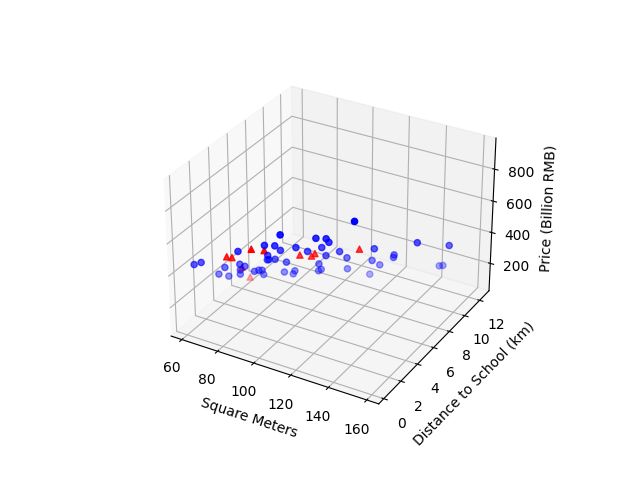
\includegraphics[width=.95\linewidth]{./figure/1(a)1.png}
			\caption{Scatter Plot of Data Distribution}
		\end{minipage}
		\begin{minipage}{.48\textwidth}
			\centering
			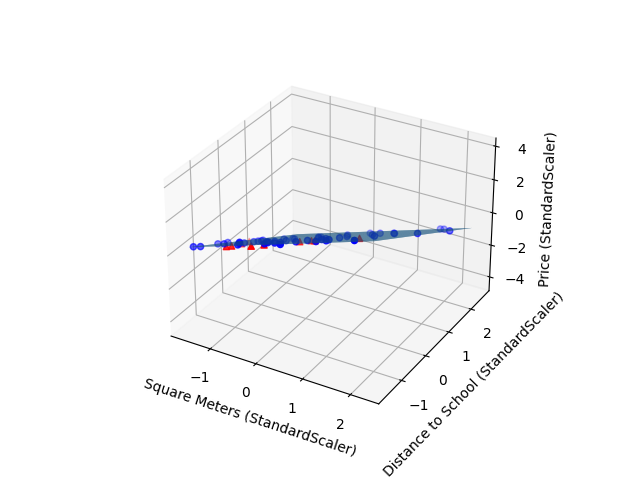
\includegraphics[width=.95\linewidth]{./figure/1(a)2.png}
			\caption{Regression Surface Plot}
		\end{minipage}
	\end{figure}
	
	To obtain the optimal regression coefficients, this study employed gradient descent. This method adjusts the parameters iteratively to minimize the loss function, typically using the root mean square error ($RMSE$) as the loss function. The iteration process of gradient descent is described as follows:
	
	\begin{enumerate}[itemsep=2pt, topsep=0pt, parsep=0pt]
	    \item \textbf{Parameter Initialization}: The initial regression coefficients (theta) are set to zero.
	    \item \textbf{Gradient Calculation}: In each iteration, the gradient of the loss function is calculated and used to update the regression coefficients.
	    \item \textbf{Parameter Update}: The parameters are adjusted using the learning rate, and the iteration continues until the maximum number of iterations is reached.
	\end{enumerate}
	
	The gradient update formula is:
	
	\vspace{-.5em}
	\begin{equation}
		\theta_j \leftarrow \theta_j - \alpha \cdot \frac{1}{m} \sum_{i=1}^{m}(h_\theta(x^{(i)}) - y^{(i)})x_j^{(i)}
		\nonumber
	\end{equation}
	
	where $h_\theta(x)$ represents the predicted value of the model, $\alpha$ is the learning rate, and $m$ is the number of training samples. During training, we recorded the current training and test errors every $100,000$ iterations and plotted the error curves as a function of the number of iterations. The error is calculated using $RMSE$, as shown in the formula below:
	
	\vspace{-.5em}
	\begin{equation}
		RMSE = \sqrt{\frac{1}{m}\sum_{i=1}^{m}(h_\theta(x^{(i)}) - y^{(i)})^2}
		\nonumber
	\end{equation}
	
	where $h_\theta(x)$ represents the predicted values of the model.
	
	\begin{figure}[htbp]
		\centering
		\begin{subfigure}{.48\textwidth}
			\centering
			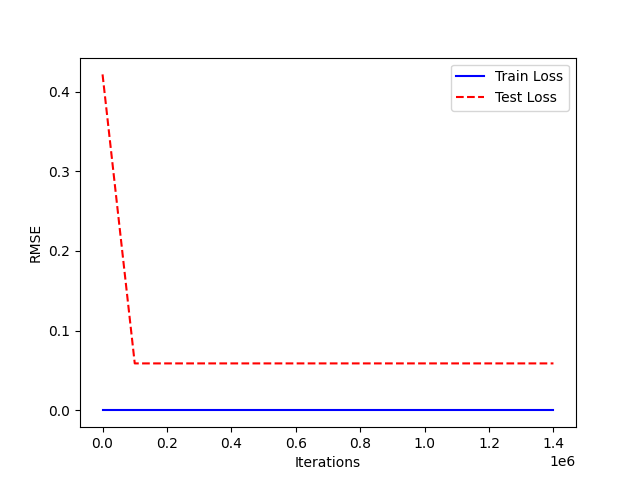
\includegraphics[width=.95\linewidth]{./figure/1(a)3.png}
			\caption{Sampling Every 100,000 Iterations}
		\end{subfigure}
		\begin{subfigure}{.48\textwidth}
			\centering
			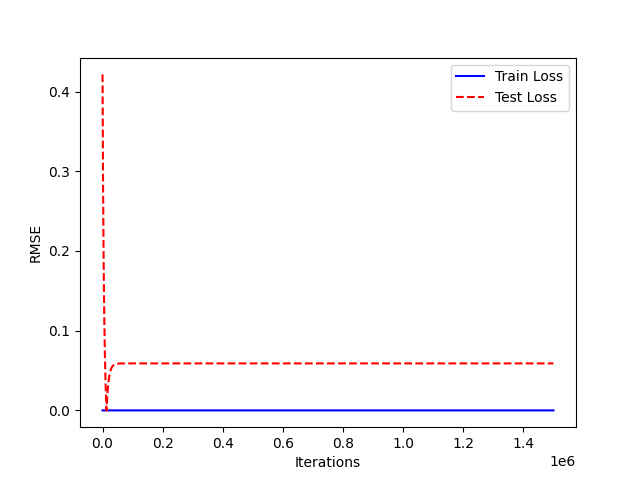
\includegraphics[width=.95\linewidth]{./figure/1(a)4.png}
			\caption{Sampling Every Each Iterations}
		\end{subfigure}
		\caption{$RMSE$ of Regression Model (learning rate = $0.00015$)}
	\end{figure}
	
	In terms of code implementation, this code used $1,500,000$ iterations and set the learning rate to $0.00015$. Every $100,000$ iterations, we sampled and plotted the changes in both training and test errors. The code is shown as \verb|Exercises1(a).py|. By observing the error curve, it can be seen that the training error continuously decreases as the number of iterations increases and gradually approaches a lower value, indicating that the model is progressively optimizing and fitting the training data. Meanwhile, the test error also shows a decreasing trend, but after approximately $10,000$ iterations, the test error begins to rise. This suggests that the model fits the training set well but shows fluctuations in performance on the test set. This phenomenon is typically associated with overfitting. Overfitting occurs when the model has learned too much from the training data, losing its ability to generalize to new data (i.e., the test data). Therefore, if error rebound is observed during training, it may be necessary to adjust the model complexity or apply regularization techniques to mitigate overfitting.
	
	\subsubsection{Question\ (b)}
	
	Based on the code and training details described in Question (a), we adjusted the learning rate and the number of iterations during model training. Given that the dataset size is only $50 + 10$, $1,500,000$ iterations seemed excessively large for this dataset. Therefore, we first assumed that with a learning rate of $0.00015$, the number of iterations needed to effectively train the model would be in the order of $10^3$. In practice, to better observe overfitting, we decided to set the training iterations to 50,000 and use this setup to monitor the error progression during the model training process.
	
	Additionally, to study the impact of different learning rates on the training process, we set the learning rates to: $0.15, 0.015, 0.0015, 0.00015, 0.000015, 0.0000015, 1.1$, and adjusted the corresponding number of iterations to ensure effective training for each learning rate. Based on our estimates, the number of iterations for each learning rate is as follows:
	
	\begin{itemize}[itemsep=2pt, topsep=0pt, parsep=0pt]
	    \item Learning rate $0.15$: 50 iterations
	    \item Learning rate $0.015$: 500 iterations
	    \item Learning rate $0.0015$: 5000 iterations
	    \item Learning rate $0.00015$: 50,000 iterations
	    \item Learning rate $0.000015$: 500,000 iterations
	    \item Learning rate $0.0000015$: 5,000,000 iterations
	    \item Learning rate $1.1$: 100 iterations
	\end{itemize}
	
	The code is shown as \verb|Exercises1(b).py|. By observing the error curves, we found that when the learning rate is less than 1, for the corresponding number of iterations, as the learning rate decreases, the error curve's descent becomes increasingly slower. This indicates that as the learning rate gradually decreases, the model's parameter updates become more refined, and the convergence process becomes more stable, but it also exhibits a gradually decelerating trend, approaching the optimal solution.
	
	However, when the learning rate exceeds 1, we observed that after a certain number of iterations, the error curve experienced an explosive increase. This phenomenon suggests that when the learning rate is too large, the magnitude of each gradient update is amplified, especially in regions with large gradients of the loss function, which can cause the model's parameters to be updated too drastically, leading to excessive updates. This over-update can result in gradient explosion, where the gradient value increases dramatically during the gradient descent process, causing large parameter updates, thus making the model diverge and fail to converge.
	
	Based on the previous observations, when the learning rate is small (e.g., below $0.00015$), the descent of the error curve becomes relatively smooth, indicating that the model gradually adapts to the training data, with both the training error and the testing error decreasing steadily. However, with a very large learning rate (e.g., $1.1$), the error curve exhibits a sharp increase, which suggests that the model fails to converge stably and exhibits divergence or oscillation. Therefore, selecting an appropriate learning rate is crucial for the stability of model training. A learning rate that is too large can lead to overfitting during training, where the model fits the training data well but loses generalization ability on the testing data. On the other hand, a smaller learning rate, although it converges more slowly, allows the model to approach the global optimum more stably, thus avoiding the risk of overfitting.
	
	\begin{figure}[htbp]
		\centering
		\begin{subfigure}{.48\textwidth}
			\centering
			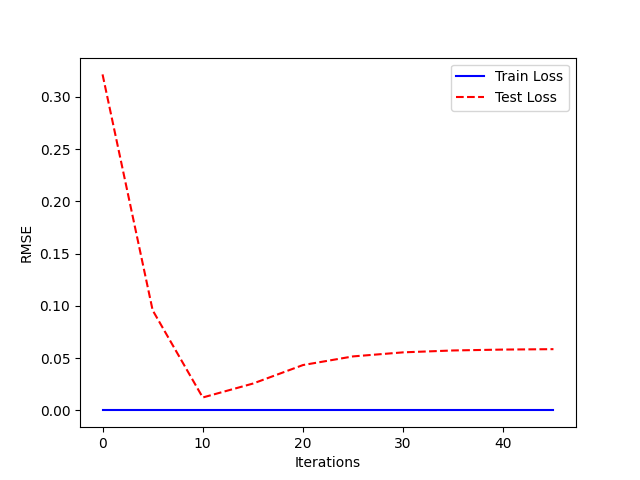
\includegraphics[width=.9\linewidth]{./figure/1(b)1.png}
			\caption{Learning Rate = $0.15$}
		\end{subfigure}
		\begin{subfigure}{.48\textwidth}
			\centering
			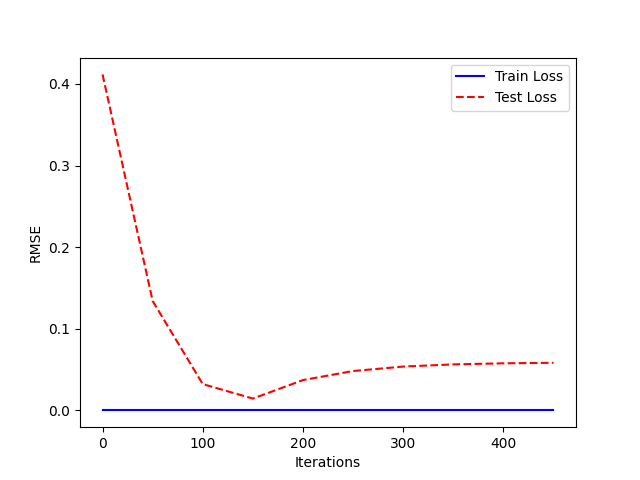
\includegraphics[width=.9\linewidth]{./figure/1(b)2.png}
			\caption{Learning Rate = $0.015$}
		\end{subfigure}
		
		\begin{subfigure}{.48\textwidth}
			\centering
			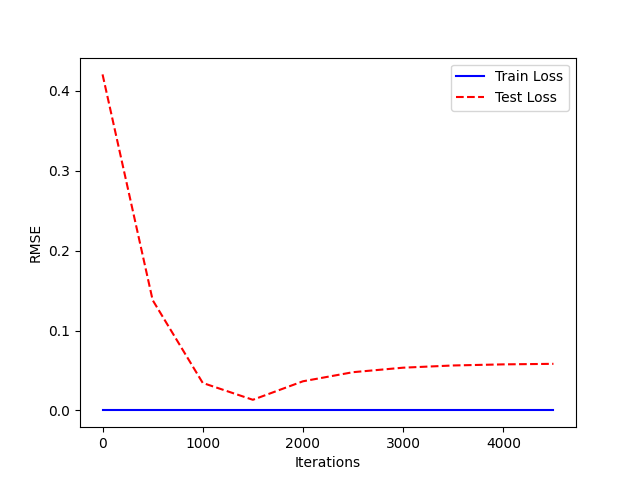
\includegraphics[width=.9\linewidth]{./figure/1(b)3.png}
			\caption{Learning Rate = $0.0015$}
		\end{subfigure}
		\begin{subfigure}{.48\textwidth}
			\centering
			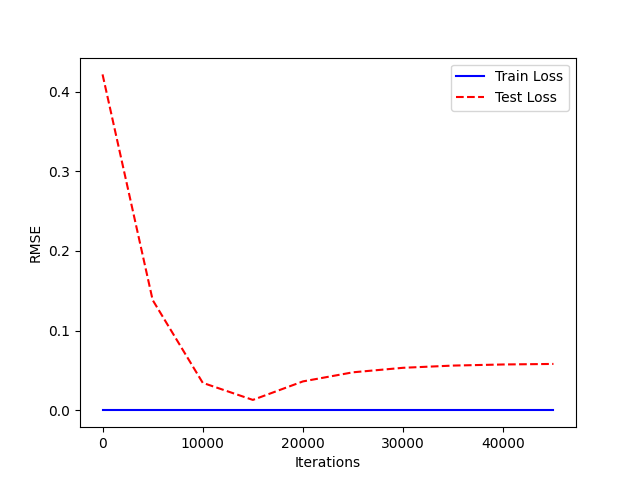
\includegraphics[width=.9\linewidth]{./figure/1(b)4.png}
			\caption{Learning Rate = $0.00015$}
		\end{subfigure}
		
		\begin{subfigure}{.48\textwidth}
			\centering
			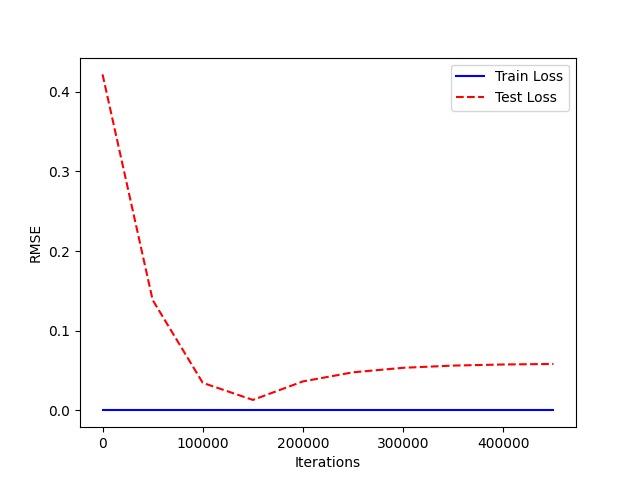
\includegraphics[width=.9\linewidth]{./figure/1(b)5.png}
			\caption{Learning Rate = $0.000015$}
		\end{subfigure}
		\begin{subfigure}{.48\textwidth}
			\centering
			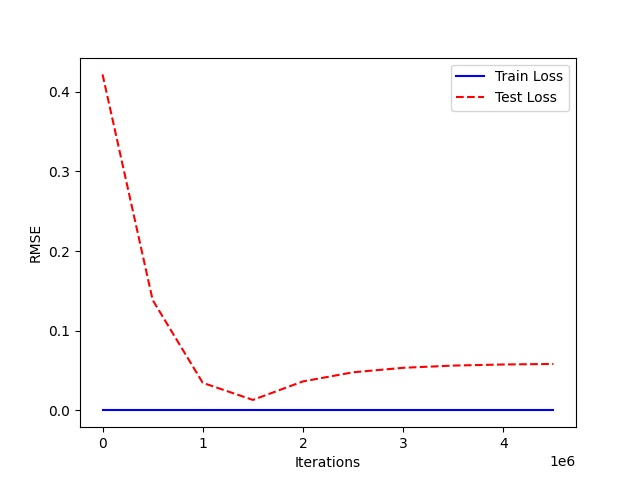
\includegraphics[width=.9\linewidth]{./figure/1(b)6.png}
			\caption{Learning Rate = $0.0000015$}
		\end{subfigure}
		\caption{$RMSE$ of Regression Model Under Different Learning Rates}
	\end{figure}
	
	\begin{figure}[htbp]
		\centering
		\begin{subfigure}{.48\textwidth}
			\centering
			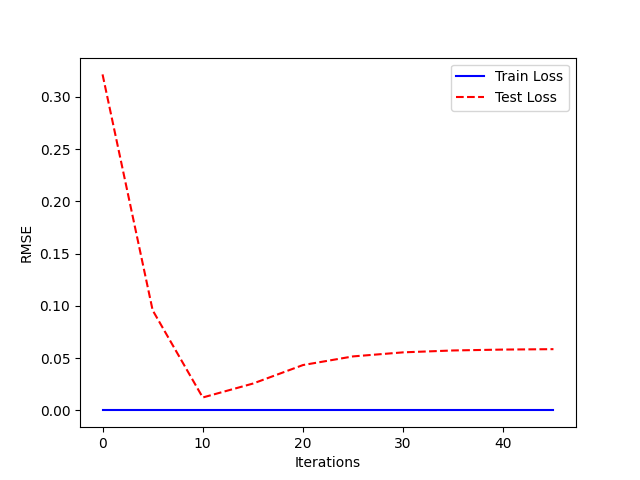
\includegraphics[width=.9\linewidth]{./figure/1(b)1.png}
			\caption{Learning Rate = $0.15$}
		\end{subfigure}
		\begin{subfigure}{.48\textwidth}
			\centering
			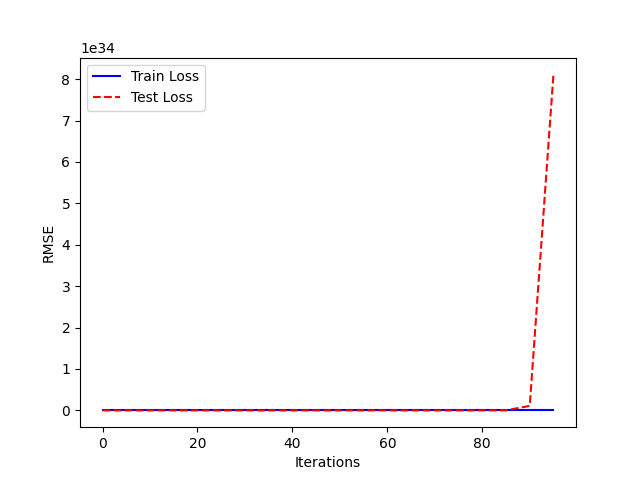
\includegraphics[width=.9\linewidth]{./figure/1(b)7.png}
			\caption{Learning Rate = $1.1$}
		\end{subfigure}
		\caption{Gradient Explosion Diagram}
	\end{figure}
	
	\subsubsection{Question(c)}
	
	In this question, we used Stochastic Gradient Descent (SGD) to train a linear regression model and solve for the optimal parameters. By monitoring the evolution of training and testing errors, we analyzed the performance of the model. Unlike Batch Gradient Descent, which updates the gradient using the entire dataset in each iteration, SGD updates the gradient using only a small subset of the data in each iteration, known as mini-batch gradient updates. This update mechanism increases the frequency of iterations and introduces randomness, thereby accelerating the training process and potentially avoiding local optima.
	
	In the experimental design, we set $1,500,000$ iterations, a learning rate of $0.00015$, and a batch size of 32, and we decided to record the training and testing errors every $100,000$ iterations. During the training process, as the number of iterations increased, the training error gradually decreased, indicating that the model was progressively learning and fitting the training data. The evolution of the testing error reflected the model’s generalization ability. The code is shown as \verb|Exercises1(c).py|. 
	
	From the observation of the training and testing error curves, we made the following conclusions:
	
	\begin{enumerate}[itemsep=2pt, topsep=0pt, parsep=0pt]
	    \item \textbf{Decreasing Training Error Trend}: As the number of iterations increased, the training error consistently decreased and approached stability, indicating that the model gradually adapted to the training data and found the appropriate parameters. With a smaller learning rate, the decrease in training error was generally smoother, as the parameter updates were slower, allowing the model to fit the training data more carefully.
	    \item \textbf{Evolution of Testing Error}: The testing error also showed a decreasing trend in the early stages, but after a certain number of iterations, it began to stabilize, and in some cases, even slightly increased. This could be due to overfitting, where the model learns the training data too well, reducing its generalization ability on the test set. Overfitting typically occurs when the model fits the training data too perfectly without being able to generalize to new, unseen data.
	    \item \textbf{Role of Learning Rate}: The choice of learning rate is critical for model training. A smaller learning rate (e.g., 0.00015) usually results in a stable training process with slower convergence, but it can avoid issues like gradient explosion and other instabilities. Larger learning rates may cause fluctuations during training, potentially leading to gradient explosion and affecting the model's convergence. In this experiment, as the learning rate decreased, both the training and testing errors stabilized, indicating that the optimization process became more detailed and stable.
	\end{enumerate}
	
	\begin{figure}[htbp]
		\centering
		\begin{subfigure}{.48\textwidth}
			\centering
			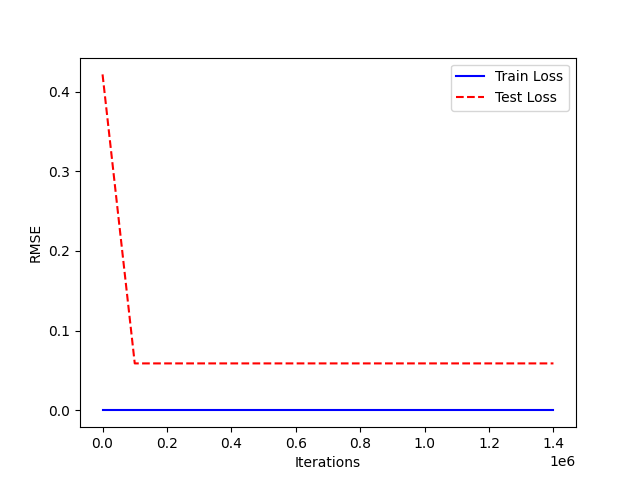
\includegraphics[width=.95\linewidth]{./figure/1(a)3.png}
			\caption{Optimized using gradient descent method}
		\end{subfigure}
		\begin{subfigure}{.48\textwidth}
			\centering
			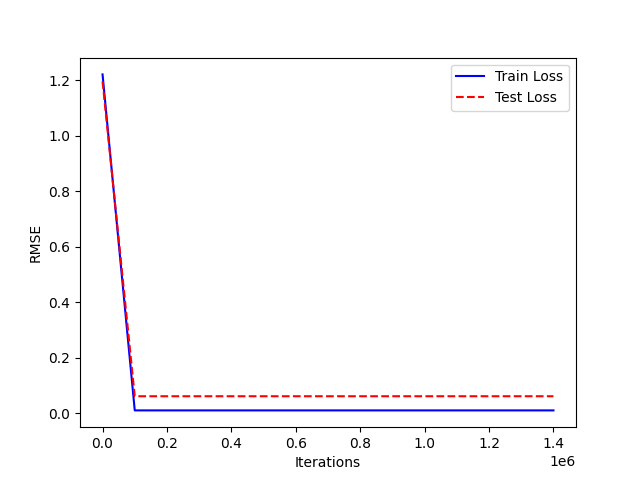
\includegraphics[width=.95\linewidth]{./figure/1(c).png}
			\caption{Optimized using Stochastic Gradient Descent}
		\end{subfigure}
		\caption{$RMSE$ of Regression Model (learning rate = $0.00015$)}
	\end{figure}
	
	Compared to Batch Gradient Descent, the advantage of Stochastic Gradient Descent lies in its use of a small subset of data in each iteration, which accelerates the parameter update process and allows for faster observation of changes in training error. Additionally, the randomness introduced by SGD in each iteration helps the model avoid getting stuck in local optima, increasing the chances of finding the global optimum. However, this randomness can also lead to more significant fluctuations in the training error curve in the early stages, requiring more iterations to stabilize.
	
	\section{Exercise Two: Logistic Regression}
	
	\subsection{Question}
	
	You will implement a logistic regression classifier and apply it to a two-class classification problem. 
	
	To get started, download the two datasets, ``\verb|dataForTrainingLogistic.txt|'' and ``\verb|data|\ \verb|ForTestingLogistic.txt|'' from the folder called ``\verb|Homework 3|''. In both of these two datasets, each instance is put per line with the first to the six columns being the features of the instance and the last column being the ground-truth label of the category (either ``$1$'' or ``$0$'') that the instance should be classified into. Each column per line is separated by a whitespace.
	
	\vspace{.5em}
	
	(a) In logistic regression, our goal is to learn a set of parameters by maximizing the conditional log likelihood of the data. Assuming you are given a dataset with $n$ training examples and $p$ features, write down a formula for the conditional log likelihood of the training data in terms of the the class labels $y^{(i)}$, the features $x^{(i)}_1, \ldots, x^{(i)}_p$, and the parameters $w_0, w_1, \ldots, w_p$, where the superscript $(i)$ denotes the sample index. This will be your objective function for gradient ascent.
	
	\vspace{.5em}
	
	(b) Compute the partial derivative of the objective function with respect to $w_0$ and with respect to an arbitrary $w_j$, i.e.~derive $\partial f / \partial w_0$ and $\partial f / \partial w_j$, where $f$ is the objective that you provided above.
	Please show all derivatives can be written in a finite sum form.
	
	\vspace{.5em}
	
	(c) Train your logistic regression classifier on the data provided in the training dataset ``\verb|dataForTrainingLogistic.txt|''. How do you design and train your logistic regression classifier? What are your optimal estimated parameters in your logistic regression classifier? Use your estimated parameters  to calculate predicted labels for the data in the testing dataset ``\verb|dataForTestingLogistic.txt|'' (Do not use the label information (the last column in the file) for testing).
	
	\vspace{.5em}
	
	(d) Report the number of misclassified examples in the testing dataset.
	
	\vspace{.5em}
	
	(e) Plot the value of the objective function on each iteration of stochastic gradient ascent, with the iteration number on the horizontal axis and the objective value on the vertical axis. Make sure to include axis labels and a title for your plot. Report the number of iterations that are required for the algorithm to converge. 
	
	\vspace{.5em}
	
	(f) Next, you will evaluate how the training and test error change as the training set size increases. For each value of $k$ in the set $\{10, 20, 30, \ldots, 380, 390, 400\}$, first choose a random subset of the training data of size $k$.  Then re-train your logistic regression classifier using the $k$ random subset of the training data you just chose, and use the estimated parameters to calculate the number of misclassified examples on both the current training set ($k$ random instances) and on the original test set ``\verb|dataForTestingLogistic.txt|''. Finally, generate a plot with two lines: in blue, plot the value of the training error against $k$, and in red, plot the value of the test error against $k$, where the error should be on the vertical axis and training set size should be on the horizontal axis. Make sure to include a legend in your plot to label the two lines. Describe what happens to the training and test error as the training set size increases, and provide an explanation for why this behavior occurs.
	
	\subsection{Answer}
	
	\subsubsection{Question(a)}
	
	In the logistic regression model, our goal is to learn a set of model parameters by maximizing the conditional log-likelihood function. Suppose we have a dataset containing $ n $ training samples and $ p $ features, where the feature vector of the $ i $-th sample is $ x^{(i)} = [x^{(i)}_1, x^{(i)}_2, \dots, x^{(i)}_p] $, and the corresponding class label is $ y^{(i)} \in \{0, 1\} $. Here, $ y^{(i)} $ represents the binary label of the $ i $-th sample (i.e., the target variable), which takes values 0 or 1, indicating whether the sample belongs to a particular class or not.
	
	In the logistic regression model, we assume that the conditional probability of each sample's label $ y^{(i)} $ is given by the following equation:
	
	\vspace{-.5em}
	\begin{equation}
		P(y^{(i)} = 1 \mid x^{(i)}; w) = \sigma(w^T x^{(i)})
		\nonumber
	\end{equation}
	
	where $ w = [w_0, w_1, \dots, w_p] $ is the vector of model parameters, including the bias term $ w_0 $ and the weights $ w_1, w_2, \dots, w_p $ corresponding to each feature $ x_1, x_2, \dots, x_p $, and $ \sigma(z) = \frac{1}{1 + e^{-z}} $ is the logistic activation function (also called the sigmoid function).
	
	To find the optimal parameters $ w $, we need to maximize the conditional log-likelihood function. The log-likelihood function is the logarithm of the likelihood of the observed data given the model parameters. Suppose we have $ n $ independent training samples, with the $ i $-th sample's label $ y^{(i)} $ and feature vector $ x^{(i)} $. The conditional log-likelihood function for the training data is then:
	
	\vspace{-.5em}
	\begin{equation}
		\ell(w) = \sum_{i=1}^{n} \left[ y^{(i)} \log(\sigma(w^T x^{(i)})) + (1 - y^{(i)}) \log(1 - \sigma(w^T x^{(i)})) \right]
		\nonumber
	\end{equation}
	
	Here, $ \sigma(w^T x^{(i)}) $ is the probability that the $ i $-th sample belongs to class 1, while $ 1 - \sigma(w^T x^{(i)}) $ is the probability that the sample belongs to class 0. Thus, for each sample, if its true label $ y^{(i)} $ is 1, we want the model to predict the sample as class 1 (i.e., $ \sigma(w^T x^{(i)}) $ should be as close to 1 as possible); if its label is 0, we want the model to predict the sample as class 0 (i.e., $ 1 - \sigma(w^T x^{(i)}) $ should be as close to 1 as possible).
	
	Therefore, the objective of the conditional log-likelihood function is to adjust the model parameters $ w $ to maximize the predicted probability for each sample, thus improving the model's fit to the data. This objective function provides the basis for optimization using gradient ascent (or gradient descent), helping us find the optimal parameters that maximize the log-likelihood function.
	
	
	\subsubsection{Question(b)}
	
	In logistic regression, our goal is to learn a set of model parameters by maximizing the conditional log-likelihood function. Suppose we have a dataset consisting of $n$ training samples, each with $p$ features, where the feature vector of the $i$-th sample is denoted as $x^{(i)} = [x_1^{(i)}, x_2^{(i)}, \dots, x_p^{(i)}]$, and the corresponding label is $y^{(i)} \in \{0, 1\}$. The model's prediction for each sample is given by the logistic function:
	
	\vspace{-.5em}
	\begin{equation}
		\sigma(w^T x^{(i)}) = \frac{1}{1 + e^{-w^T x^{(i)}}}
		\nonumber
	\end{equation}
	
	where $ w = [w_0, w_1, \dots, w_p] $ is the parameter vector of the model, with $ w_0 $ as the bias term and $ w_1, w_2, \dots, w_p $ as the weights associated with the features $ x_1, x_2, \dots, x_p $. The goal is to maximize the log-likelihood function (log-likelihood), which is expressed as:
	
	\vspace{-.5em}
	\begin{equation}
		f(w) = \sum_{i=1}^{n} \left[ y^{(i)} \log(\sigma(w^T x^{(i)})) + (1 - y^{(i)}) \log(1 - \sigma(w^T x^{(i)})) \right]
		\nonumber
	\end{equation}
	
	\vspace{.5em}
	
	\textbf{1. Partial Derivative with Respect to $w_0$}
	
	\vspace{.5em}
	
	First, we compute the partial derivative of the objective function $f(w)$ with respect to the bias term $w_0$. To simplify, we first compute the derivative of each term with respect to $w_0$. The log-likelihood function for each term is given by:
	
	\vspace{-.5em}
	\begin{equation}
		y^{(i)} \log(\sigma(w^T x^{(i)})) + (1 - y^{(i)}) \log(1 - \sigma(w^T x^{(i)}))
		\nonumber
	\end{equation}
	
	When differentiating with respect to $w_0$, we apply the chain rule, noting that the bias term $w_0$ only affects the inner product $w^T x^{(i)}$. The derivative of the logistic function $ \sigma(z) $ is given by:
	
	\vspace{-.5em}
	\begin{equation}
		\sigma'(z) = \sigma(z)(1 - \sigma(z))
		\nonumber
	\end{equation}
	
	Since $x_0^{(i)} = 1$, representing the bias term, the partial derivative of $f(w)$ with respect to $w_0$ is:
	
	\vspace{-.5em}
	\begin{equation}
		\begin{aligned}
			\frac{\partial f(w)}{\partial w_0} = & \sum_{i=1}^{n} \Bigg[ \left( y^{(i)} \cdot \frac{1}{\sigma(w^T x^{(i)})} \cdot \sigma'(w^T x^{(i)}) \cdot 1 \right) \\
			&+ \left( (1 - y^{(i)}) \cdot \frac{1}{1 - \sigma(w^T x^{(i)})} \cdot \sigma'(w^T x^{(i)}) \cdot 1 \right) \Bigg]
		\end{aligned}
		\nonumber
	\end{equation}
	
	Simplifying this, the final expression for the partial derivative with respect to $w_0$ is:
	
	\vspace{-.5em}
	\begin{equation}
		\frac{\partial f(w)}{\partial w_0} = \sum_{i=1}^{n} \left( \sigma(w^T x^{(i)}) - y^{(i)} \right)
		\nonumber
	\end{equation}
	
	This expression represents the gradient of the objective function with respect to the bias term $w_0$, which measures the error between the predicted probability and the true label for each sample.
	
	\vspace{.5em}
	
	\textbf{2. Partial Derivative with Respect to $w_j$}
	
	\vspace{.5em}
	
	Next, we compute the partial derivative of the objective function $f(w)$ with respect to any $w_j$ (where $j = 1, 2, \dots, p$). Similar to the case of $w_0$, we apply the chain rule for differentiation. The log-likelihood function for each term with respect to $w_j$ is:
	
	\vspace{-.5em}
	\begin{equation}
		y^{(i)} \log(\sigma(w^T x^{(i)})) + (1 - y^{(i)}) \log(1 - \sigma(w^T x^{(i)}))
		\nonumber
	\end{equation}
	
	For each term involving $x_j^{(i)}$, we again apply the chain rule and relate the change in $w_j$ to the corresponding feature $x_j^{(i)}$. The final expression for the partial derivative with respect to $w_j$ is:
	
	\vspace{-.5em}
	\begin{equation}
		\begin{aligned}
			\frac{\partial f(w)}{\partial w_j} = & \sum_{i=1}^{n} \Bigg[ \left( y^{(i)} \cdot \frac{1}{\sigma(w^T x^{(i)})} \cdot \sigma'(w^T x^{(i)}) \cdot x_j^{(i)} \right) \\
			&+ \left( (1 - y^{(i)}) \cdot \frac{1}{1 - \sigma(w^T x^{(i)})} \cdot \sigma'(w^T x^{(i)}) \cdot x_j^{(i)} \right) \Bigg]
		\end{aligned}
		\nonumber
	\end{equation}
	
	Simplifying, the final expression for the partial derivative with respect to $w_j$ is:
	
	\vspace{-.5em}
	\begin{equation}
		\frac{\partial f(w)}{\partial w_j} = \sum_{i=1}^{n} \left( \sigma(w^T x^{(i)}) - y^{(i)} \right) \cdot x_j^{(i)}
		\nonumber
	\end{equation}
	
	This result represents the gradient of the objective function with respect to $w_j$, reflecting how each feature $x_j^{(i)}$ contributes to the loss function and indicating how the weight $w_j$ should be adjusted based on the feature's value.
	
	\subsubsection{Question(c)}
	
	To achieve the stated goal, a logistic regression classifier based on the Stochastic Gradient Descent (SGD) algorithm is constructed. The design and training process of this classifier are detailed as follows:
	
	\begin{enumerate}[itemsep=2pt, topsep=0pt, parsep=0pt]
		\item \textbf{Data Preprocessing}: First, the training and testing datasets are imported using the \verb|np.loadtxt()| function. The training dataset is stored in an array named \verb|train|, while the testing dataset is stored in an array named \verb|test|. Subsequently, the features (the first six columns) of the training dataset are extracted into the \verb|x_train| array, and the corresponding labels are stored in the \verb|y_train| array. Similarly, the features and labels of the testing dataset are stored in the \verb|x_test| and \verb|y_test| arrays, respectively. These datasets serve as the input variables for the logistic regression model.
		
		\item \textbf{Introducing the Bias Term}: Logistic regression models typically require the introduction of a bias term (or intercept). Therefore, a column of ones is added to the feature matrices \verb|X_train| and \verb|X_test| in both the training and testing datasets. This ensures that each feature vector takes the form of $[1, x_1, x_2, \dots, x_p]$, where $x_1, x_2, \dots , x_p$ represent the original features. This operation is carried out using the \verb|np.concatenate()| function.
		
		\item \textbf{Defining the Logistic Regression Function and Gradient Descent Algorithm}
		\begin{itemize}[itemsep=2pt, topsep=0pt, parsep=0pt]
		    \item The \verb|logistic()| function implements the activation function for logistic regression, $\sigma(z) = \frac{1}{1 + \exp(-z)}$, which converts the model's linear output into a probability value.
		    \item The \verb|GD()| function uses the stochastic gradient descent algorithm to train the logistic regression model. In each iteration, the model's predictions are computed based on the current parameter vector $\theta$, and the gradient of the loss function is calculated to update the parameters. The loss function consists of the cross-entropy loss and an L2 regularization term. After each parameter update, the training and testing set losses are recorded for later analysis of the model's training process.
		\end{itemize}
		
		\item \textbf{Model Training and Prediction}: During the training phase, the \verb|GD()| function is called with predefined hyperparameters, including the number of iterations (\verb|num_steps|), learning rate (\verb|learning_rate|), and regularization coefficient (\verb|l2_coef}|. This function returns the learned parameters $\theta$, along with the training and testing set losses. After training is complete, the obtained parameters $\theta$ are used to make predictions on the testing set. Specifically, the logistic regression model calculates the predicted probabilities for each sample in the testing set. A predicted label is assigned based on whether the probability is greater than or equal to $0.5$. Finally, the prediction accuracy is calculated by comparing the predicted labels to the true labels of the testing set, and the number of misclassified samples is counted.
		
		\item \textbf{Plotting the Loss Curves}: To visually demonstrate the model's training performance, the code uses \verb|matplotlib| to plot curves showing how the training and testing losses change with each iteration. This allows for a clear observation of the loss trends during the training process, providing insight into the model's convergence.
	\end{enumerate}
	
	Ultimately, the model outputs the prediction accuracy on the testing set, the regression coefficients $\theta$, and the number of misclassified samples. The regression coefficients $\theta$ are the optimal parameters estimated through the gradient descent algorithm, and these parameters define the decision boundary of the logistic regression model, directly influencing the prediction of the classification results. The code is shown as \verb|Exercises2(c)(d)(e).py|.
	
	\subsubsection{Question(d)}
	
	To achieve the goal of this task, the number of misclassified samples is calculated using the following formula and method:
	
	\vspace{-.5em}
	\begin{equation}
		\text{errors} = \sum_{i=1}^{n} \left( y_{\text{pred}}^{(i)} \neq y_{\text{test}}^{(i)} \right)
		\nonumber
	\end{equation}
	
	This formula compares the predicted labels $ y_{\text{pred}} $ with the true labels $ y_{\text{test}} $ for each sample and counts the number of mismatches, which corresponds to the number of misclassified samples. Specifically, for each sample $ i $, if the predicted label differs from the true label (i.e., $ y_{\text{pred}}^{(i)} \neq y_{\text{test}}^{(i)} $), it indicates that the sample has been misclassified. By summing over all the samples, the total number of misclassified samples is obtained. The result is then printed to the console to help the user understand how many samples in the test dataset have predicted labels that differ from the actual labels. The code is shown as \verb|Exercises2(c)(d)(e).py|, and shown as the result, the number of misclassified samples is 0.
	
	During the model training and prediction phase, the optimal parameters $ \theta $ are first learned from the training dataset, and then these parameters are used to make predictions on the test dataset. For each test sample, the model calculates the predicted probability and classifies the sample as 0 or 1 based on a threshold (typically 0.5). Next, by comparing the predicted labels with the true labels, the number of misclassified samples is computed. In this way, we can quantify the model's classification performance on the test set and further analyze its effectiveness.
	
	\subsubsection{Question(e)}
	
	By plotting the relevant graphs, it can be observed that the algorithm causes the model to converge after approximately $100$ training epochs, with both the training and test errors achieving convergence. This means that the algorithm requires about 100 iterations to reach convergence. Specifically, this process involves training the model using the Stochastic Gradient Descent (SGD) method, where the model parameters are iteratively updated by minimizing the loss function. In this task, the loss function takes into account both the cross-entropy loss and the L2 regularization term to prevent overfitting. By recording the training and test losses for each epoch during the training process, we can plot the loss curves, providing a visual representation of the model's performance throughout the training. Ultimately, the model's prediction accuracy and regression coefficients are calculated and output to assess its performance. The code is shown as \verb|Exercises2(c)(d)(e).py|.

	\begin{figure}[htbp]
		\centering
		\centering
		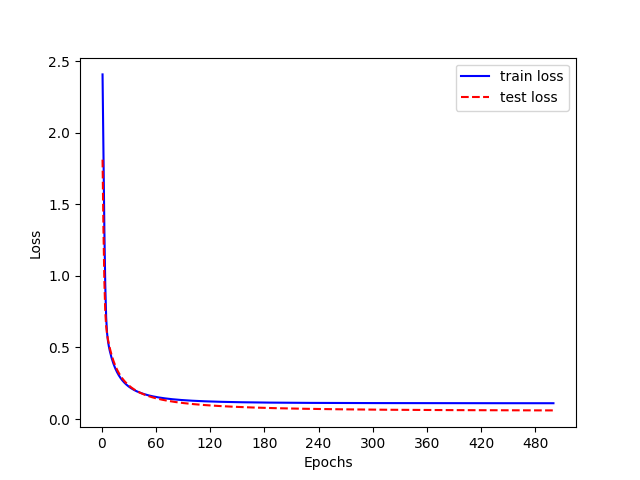
\includegraphics[width=.6\linewidth]{./figure/2-1.png}
		\caption{Loss During Gradient Descent}
	\end{figure}
	
	\subsubsection{Question(f)}
	
	The code was written according to the requirements of the task, and the chart was generated as requested. The code is shown as \verb|Exercises2(f).py|. By analyzing the chart, it can be observed that the training error converges to zero when the training set size is approximately 30, and the test error also converges to zero at the same time. This indicates that the model performs well on both the training and test sets, without overfitting or underfitting. However, in the training set size ranges of approximately 140-170, 180-200, and 320-340, the training error fluctuates, rising from 0 to 1 and then decreasing back to 0. These fluctuations may be caused by the following reasons:
	
	\begin{enumerate}[itemsep=2pt, topsep=0pt, parsep=0pt]
	    \item \textbf{Randomness of the dataset}: Since each iteration involves randomly selecting $k$ samples from the original dataset as the training set, in certain specific training set size ranges, the randomly selected samples may contain some noise or outliers. This can cause the model's training error to temporarily increase in those ranges. As the iterations continue, the model may gradually adapt to these noise or outliers, causing the training error to decrease again.
	    \item \textbf{Convergence characteristics of gradient descent}: At certain training set sizes, the gradient descent algorithm may require more iterations to find the minimum of the loss function, or it may oscillate around a local minimum, leading to fluctuations in the training error.
	    \item \textbf{Effect of the regularization term}: Since an L2 regularization term is used, the impact of the regularization term on the model may change as the training set size varies, which could cause fluctuations in the training error in some ranges.
	    \item \textbf{Model complexity and data size mismatch}: In certain training set size ranges, the complexity of the model may not match the amount of available data, leading to a temporary decline in model performance during training.
	\end{enumerate}
	
	Overall, although the training error fluctuates in some ranges, the model ultimately converges to a low error on both the training and test sets, indicating that the model has good generalization ability.
	
	\begin{figure}[htbp]
		\centering
		\centering
		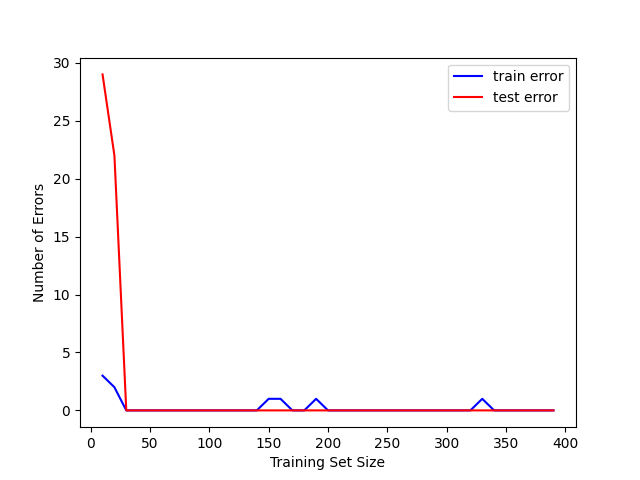
\includegraphics[width=.6\linewidth]{./figure/2-2.png}
		\caption{Training and Test Errors As A Function of Training Set Size}
	\end{figure}
	
\end{document}